\documentclass[tikz,border=6pt]{standalone}
\usepackage{xcolor}
\begin{document}
% Canonical ch-diagram for 10_1^0,1
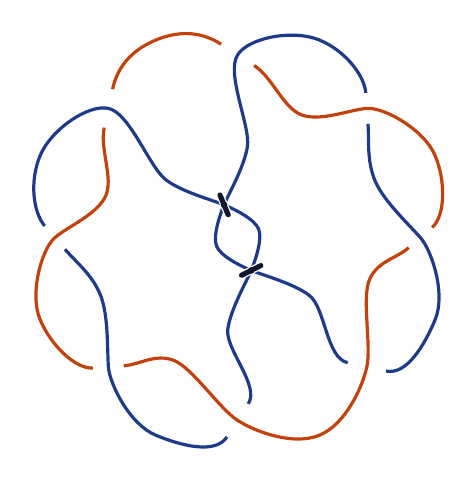
\begin{tikzpicture}[line join=round]
  \definecolor{skcomp0}{RGB}{30,58,138}
  \definecolor{skcomp1}{RGB}{194,65,12}
  \definecolor{skmark}{RGB}{15,23,42}
  \draw[skcomp0, line width=1.15pt, line cap=butt] (-2.1927,-0.0945) .. controls (-2.0481,-0.2614) and (-1.8507,-0.4131) .. (-1.7448,-0.6689);
  \draw[skcomp1, line width=1.15pt, line cap=butt] (-1.6940,1.4512) .. controls (-1.7533,1.1768) and (-1.5718,0.8077) .. (-1.6778,0.5786);
  \draw[skcomp0, line width=1.15pt, line cap=butt] (-2.4497,0.2022) .. controls (-2.5943,0.3691) and (-2.6462,0.7629) .. (-2.5093,1.0932);
  \draw[skcomp1, line width=1.15pt, line cap=butt] (-1.8371,-1.6015) .. controls (-2.0574,-1.6173) and (-2.3725,-1.3159) .. (-2.5093,-0.9855);
  \draw[skcomp0, line width=1.15pt, line cap=butt] (-0.1352,-2.4771) .. controls (-0.2789,-2.7000) and (-0.7090,-2.5923) .. (-1.0394,-2.4555);
  \draw[skcomp1, line width=1.15pt, line cap=butt] (-1.4456,-1.5735) .. controls (-1.2375,-1.5585) and (-1.0522,-1.4166) .. (-0.8153,-1.5036);
  \draw[skcomp0, line width=1.15pt, line cap=butt] (0.1352,-2.0576) .. controls (0.2874,-1.8216) and (-0.1638,-1.3614) .. (-0.1246,-1.1038);
  \draw[skcomp1, line width=1.15pt, line cap=butt] (-1.5886,1.9391) .. controls (-1.5326,2.1983) and (-1.3698,2.4263) .. (-1.0394,2.5632);
  \draw[skcomp1, line width=1.15pt, line cap=butt] (-0.2098,2.5103) .. controls (-0.4327,2.6540) and (-0.7090,2.7000) .. (-1.0394,2.5632);
  \draw[skcomp1, line width=1.15pt, line cap=butt] (0.2098,2.2398) .. controls (0.4458,2.0877) and (0.5784,1.6983) .. (0.8153,1.6113);
  \draw[skcomp0, line width=1.15pt, line cap=butt] (1.6273,1.8910) .. controls (1.6115,2.1112) and (1.3698,2.4263) .. (1.0394,2.5632);
  \draw[skcomp0, line width=1.15pt, line cap=butt] (1.6554,1.4994) .. controls (1.6711,1.2791) and (1.6388,1.0323) .. (1.7448,0.7766);
  \draw[skcomp1, line width=1.15pt, line cap=butt] (2.4695,0.1824) .. controls (2.6365,0.3269) and (2.6462,0.7629) .. (2.5093,1.0932);
  \draw[skcomp1, line width=1.15pt, line cap=butt] (2.1728,-0.0747) .. controls (2.0152,-0.2112) and (1.7838,-0.2419) .. (1.6778,-0.4709);
  \draw[skcomp0, line width=1.15pt, line cap=butt] (1.8853,-1.6402) .. controls (2.1445,-1.6962) and (2.3725,-1.3159) .. (2.5093,-0.9855);
  \draw[skcomp0, line width=1.15pt, line cap=butt] (1.3974,-1.5348) .. controls (1.1229,-1.4755) and (1.1165,-0.8311) .. (0.9067,-0.6766);
  \draw[skcomp0, line width=1.15pt, line cap=round] (-1.6413,-1.5875) .. controls (-1.6571,-1.3672) and (-1.6388,-0.9246) .. (-1.7448,-0.6689);
  \draw[skcomp1, line width=1.15pt, line cap=round] (-2.3212,0.0538) .. controls (-2.1636,0.1904) and (-1.7838,0.3495) .. (-1.6778,0.5786);
  \draw[skcomp0, line width=1.15pt, line cap=round] (-1.6413,1.6952) .. controls (-1.9005,1.7512) and (-2.3725,1.4236) .. (-2.5093,1.0932);
  \draw[skcomp1, line width=1.15pt, line cap=round] (-2.3212,0.0538) .. controls (-2.4881,-0.0907) and (-2.6462,-0.6552) .. (-2.5093,-0.9855);
  \draw[skcomp0, line width=1.15pt, line cap=round] (-1.6413,-1.5875) .. controls (-1.6255,-1.8077) and (-1.3698,-2.3186) .. (-1.0394,-2.4555);
  \draw[skcomp1, line width=1.15pt, line cap=round] (0.0000,-2.2673) .. controls (-0.2360,-2.1152) and (-0.5784,-1.5906) .. (-0.8153,-1.5036);
  \draw[skcomp0, line width=1.15pt, line cap=round] (0.1725,-0.3625) .. controls (0.1135,-0.5049) and (-0.0855,-0.8461) .. (-0.1246,-1.1038);
  \draw[skcomp1, line width=1.15pt, line cap=round] (0.0000,-2.2673) .. controls (0.2229,-2.4110) and (0.7090,-2.5923) .. (1.0394,-2.4555);
  \draw[skcomp1, line width=1.15pt, line cap=round] (1.6413,-1.5875) .. controls (1.5853,-1.8467) and (1.3698,-2.3186) .. (1.0394,-2.4555);
  \draw[skcomp0, line width=1.15pt, line cap=round] (-1.6413,1.6952) .. controls (-1.3669,1.6359) and (-1.1165,0.9388) .. (-0.9067,0.7843);
  \draw[skcomp0, line width=1.15pt, line cap=round] (-0.1725,0.4702) .. controls (-0.3148,0.5292) and (-0.6968,0.6297) .. (-0.9067,0.7843);
  \draw[skcomp0, line width=1.15pt, line cap=round] (0.0000,2.3750) .. controls (-0.1521,2.1390) and (0.1638,1.4691) .. (0.1246,1.2115);
  \draw[skcomp0, line width=1.15pt, line cap=round] (-0.1725,0.4702) .. controls (-0.1135,0.6126) and (0.0855,0.9538) .. (0.1246,1.2115);
  \draw[skcomp1, line width=1.15pt, line cap=round] (1.6413,1.6952) .. controls (1.4333,1.6803) and (1.0522,1.5243) .. (0.8153,1.6113);
  \draw[skcomp0, line width=1.15pt, line cap=round] (0.0000,2.3750) .. controls (0.1437,2.5979) and (0.7090,2.7000) .. (1.0394,2.5632);
  \draw[skcomp0, line width=1.15pt, line cap=round] (2.3212,0.0538) .. controls (2.1766,0.2207) and (1.8507,0.5208) .. (1.7448,0.7766);
  \draw[skcomp1, line width=1.15pt, line cap=round] (1.6413,1.6952) .. controls (1.8616,1.7110) and (2.3725,1.4236) .. (2.5093,1.0932);
  \draw[skcomp1, line width=1.15pt, line cap=round] (1.6413,-1.5875) .. controls (1.7006,-1.3130) and (1.5718,-0.7000) .. (1.6778,-0.4709);
  \draw[skcomp0, line width=1.15pt, line cap=round] (2.3212,0.0538) .. controls (2.4658,-0.1131) and (2.6462,-0.6552) .. (2.5093,-0.9855);
  \draw[skcomp0, line width=1.15pt, line cap=round] (0.1725,-0.3625) .. controls (0.3148,-0.4215) and (0.6968,-0.5221) .. (0.9067,-0.6766);
  \draw[skcomp0, line width=1.15pt, line cap=round] (0.1725,-0.3625) .. controls (0.2282,-0.2281) and (0.3180,0.0399) .. (0.2665,0.1642);
  \draw[skcomp0, line width=1.15pt, line cap=round] (-0.1725,0.4702) .. controls (-0.0380,0.4146) and (0.2150,0.2886) .. (0.2665,0.1642);
  \draw[skcomp0, line width=1.15pt, line cap=round] (0.1725,-0.3625) .. controls (0.0380,-0.3069) and (-0.2150,-0.1809) .. (-0.2665,-0.0566);
  \draw[skcomp0, line width=1.15pt, line cap=round] (-0.1725,0.4702) .. controls (-0.2282,0.3358) and (-0.3180,0.0678) .. (-0.2665,-0.0566);
  \draw[white, line width=2.8pt, line cap=round] (0.0500,-0.4239) -- (0.2949,-0.3012);
  \draw[skmark, line width=1.85pt, line cap=round] (0.0500,-0.4239) -- (0.2949,-0.3012);
  \fill[skmark] (0.1725,-0.3625) circle (1.2pt);
  \draw[white, line width=2.8pt, line cap=round] (-0.2249,0.5968) -- (-0.1201,0.3437);
  \draw[skmark, line width=1.85pt, line cap=round] (-0.2249,0.5968) -- (-0.1201,0.3437);
  \fill[skmark] (-0.1725,0.4702) circle (1.2pt);
\end{tikzpicture}
\end{document}
